%SourceDoc ../YourName-Dissertation.tex
\vspace*{-80mm}
\chapter{The Euler Equations} \label{chapter2:euler_equations}
	
	The finite volume structure in COBRA-TF in figure \ref{fig:CTF-Cells} is for
	a one-dimmensional channel in the axial direction with $n$ number of cells.
	The first and last cells at $0$ and $n+1$ are ghost cells and act as the
	boundary conditions for the problem. Pressure, enthalpy, and density are
	averaged over the cell volume and are located at the center of the cell.
	Mass flow rate and velocity are located at the faces in between cells. The
	cells are represented with an index $i$, and the faces with indexes of
	$i+\frac{1}{2}$ or $i-\frac{1}{2}$. This project will initially focus
	on this 1-D configuration. Usually the code is three dimensional, with
	channels connecting to each other in two more dimmensions. Fully 3-D
	equations will be considered in future work.
	
	\begin{figure}[!h]
		\centering
		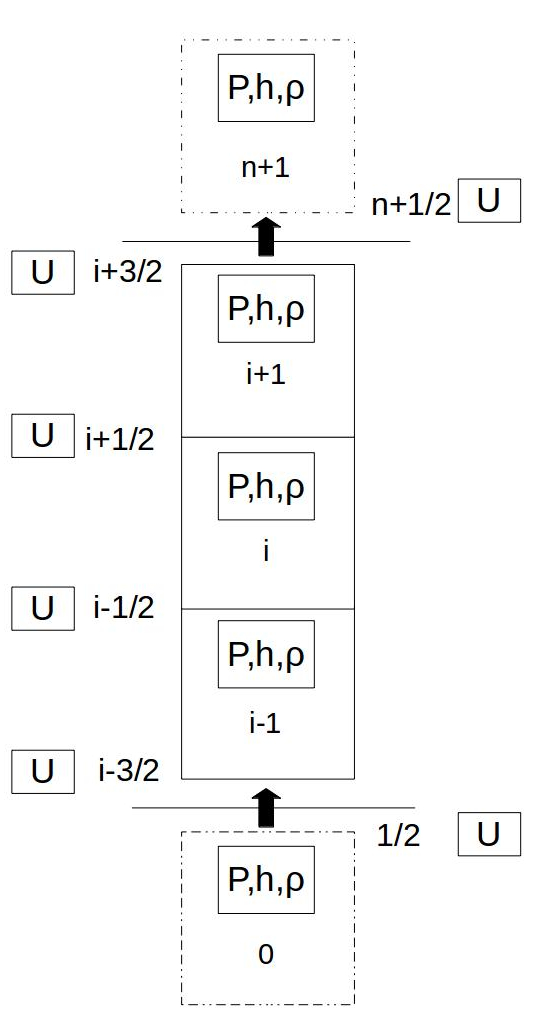
\includegraphics[width=0.30\textwidth]{images/CTF-Cells}
		
		\caption{The finite volume structure for COBRA-TF}
		\label{fig:CTF-Cells}
	\end{figure}

	The thermal hydraulics of a LWR core is an important part of nuclear
	reactor desigin. COBRA-TF solves 8 conservation equations for liquid,
	entrained droplet, and vapor phases of water boiling within the rod structure
	of a LWR reactor core \cite{CTF_Theory}. Currently, the conservation
	equations analytically reduce into a pressure matrix in a semi-implicit
	method with rod temperatures solved for explicitly. This work involves
	representing the 1-D single phase liquid conservation equations and calculated 
	variables in a residual formulation. The full jacobian matrix can then be
	built numerically, and  can then either be reduced to a pressure matrix or
	solved directly. Verification of the residuals was done by comparing
	calculated results to analytical solutions for isokinetic advection and shock
	tube problems. For each verification problem, a scaling study of the
	truncation error was compared to the predicted behaviour derived from modified
	equation analysis using Richardson extrapolation. Further work was then
	applied to represent 1-D heat conduction within the heater rods. Some initial
	work was done to allow the code to solve either semi-implicitly, or fully impicitly.
    The single phase Euler partial differential equations for mass
    \eqref{eq:pde_mass}, momentum \eqref{eq:pde_momentum}, and energy
    \eqref{eq:pde_energy} corresond to the unknown variables density $\rho$,
    velocity $u$, pressure $P$, and enthalpy $h$. The first terms in each of the
    equations are temporal terms. The rest of the terms are steady state spatial
    terms. 
    
    \begin{equation}
    	\label{eq:pde_mass}
    	\frac{ \partial \rho}{\partial t} + \bigtriangledown \rho u = 0
    \end{equation}
    
    \begin{equation}
    	\label{eq:pde_momentum}
    	\frac{ \partial \rho u}{\partial t} + \bigtriangledown \rho u^{2} +
    	\bigtriangledown P - \rho g  = 0
    \end{equation}
    
    \begin{equation}
    	\label{eq:pde_energy}
    	\frac{ \partial \rho h}{\partial t} -
    	\frac{ \partial  P}{\partial t} + 
    	\bigtriangledown ( \rho  u h )%  -
    	%u \frac{ \partial  P}{\partial x}
    	= 0
    \end{equation}
    
    The 1-D formulation of the Euler Equations will assume a direction $x$ as shown
    in the 1-D mass equation \eqref{eq:1-D_mass}. The momentum and energy equations
    are represented in a non-conservative form as shown in equations
    \eqref{eq:1-D_momentum_long} and \eqref{eq:1-D_energy_long}. The momentum
    equation contains a term that has a product of the left hand side of the 1-D
    mass equation. This terms can therefore be dropped since it is equivalent
    to zero, and the entire equation can be divided by density to give a simpler
    form of the momentum equation \eqref{eq:1-D_momentum}.
    
    \begin{equation}
    	\label{eq:1-D_mass}
    	\dfrac{ \partial \rho }{ \partial t} +
    	\dfrac{ \partial \rho u}{\partial x} = 0
    \end{equation}
    
    \begin{equation}
    	\label{eq:1-D_momentum_long}
    	\rho \dfrac{ \partial u }{ \partial t } + 
    	u \left(  \dfrac{ \partial \rho }{ \partial t } +
    	          \dfrac{ \partial \rho u }{\partial x} \right) +
    	\rho u \dfrac{ \partial u}{ \partial x} + 
    	\dfrac{ \partial P}{ \partial x}   - \rho g
    	= 0
    \end{equation}
    
    \begin{equation}
    	\label{eq:1-D_momentum}
    	\dfrac{ \partial u }{ \partial t } + 
    	u \dfrac{ \partial u }{ \partial x } + 
    	\dfrac{1}{ \rho } \dfrac{ \partial P }{ \partial x } - g  
    	= 0
    \end{equation}
    
    \begin{equation}
    	\label{eq:1-D_energy_long}
    	\rho \frac{ \partial  h}{\partial t} -
    	     \frac{ \partial  P}{\partial t} + 
    	h    \frac{ \partial  \rho}{\partial t} +
    	\rho u \frac{ \partial h }{ \partial x} +
    	h    \frac{ \partial \rho u }{ \partial x} 
    	= 0
    \end{equation}
    
    The 1-D equations are then evaluated at a position index $ i $ and a certian time
    $n$ in order to solve for the next time value of $n+1$. In the mass equation
    \eqref{eq:FD_mass}, the velocities are located at the cell faces
    $i+\frac{1}{2}$ and $i-\frac{1}{2}$. The density at a corresponding face is
    either upwinded $\dot{\rho}_{i+\frac{1}{2}}^{n}$, or averaged
    $\bar{\rho}_{i+\frac{1}{2}}^{n}$. In equation \eqref{eq:FD_momentum}, the
    derivative $\frac{ \partial u}{ \partial x}$ is upwinded assuming that the
    flow is positive. In the energy equation, \eqref{eq:FD_energy} the enthalpy
    values in the first spatial term are upwinded and shown here assuming a
    positive velocity. The equation of state \eqref{eq:EOS} solves for density
    assuming that it is a linear combination of changes due to pressure and
    enthalpy. The partial derivatives in the equation are calculated from
    steam tables as functions of old time pressure and enthalpy. 
    
    \begin{equation}
    	\label{eq:FD_mass}
    	\frac{ \rho_{i}^{n+1}-\rho_{i}^{n}}{ \Delta t} +
    	\frac{ \dot{\rho}_{i+\frac{1}{2}}^{n} u_{i+\frac{1}{2}}^{n+1}  -
    	\dot{\rho}_{i-\frac{1}{2}}^{n}  u_{i-\frac{1}{2}}^{n+1} }{\Delta x}
    	 = 0
    \end{equation}
    
    \begin{equation}
    	\label{eq:FD_momentum}
    	\frac{  u_{i+\frac{1}{2}}^{n+1} - u_{i+\frac{1}{2}}^{n} }{ \Delta t } + 
    	u_{i+\frac{1}{2}}^{n} \left( \frac{  u_{i+\frac{1}{2}}^{n} -
    	u_{i-\frac{1}{2}}^{n}}{ \Delta x} \right) +
    	\frac{1}{\bar{\rho}_{i+\frac{1}{2}}^{n} } 
    	\frac{ P_{i+1}^{n+1} -P_{i}^{n+1} }{ \Delta x } - g
    	= 0
    \end{equation}
    
    \begin{equation}
    	\label{eq:FD_energy}
    	\rho_{i}^{n} \frac{ h_{i}^{n+1} - h_{i}^{n}}{\Delta t} + 
    	h_{i}^{n} \frac{ \rho_{i}^{n+1} - \rho_{i}^{n}}{\Delta t} -
    	\frac{P_{i}^{n+1}-P_{i}^{n}}{\Delta t}+
    	\left( \rho u \right)_{i}^{n} 
    		\frac{   h _{i}^{n}  - h _{i-1}^{n} }{\Delta x} +
    	h _{i}^{n} \frac{ \dot{\rho}_{i+\frac{1}{2}}^{n} u_{i+\frac{1}{2}}^{n+1}  -
    	\dot{\rho}_{i-\frac{1}{2}}^{n}  u_{i-\frac{1}{2}}^{n+1} }{\Delta x}
    	= 0
    \end{equation}
    
    \begin{equation}
    	\label{eq:EOS}
    	\rho_{i}^{n+1} - \rho_{i}^{n} = 
    	\left( \frac{ \partial \rho }{\partial P} \right) 
    	\left( P_{i}^{n+1} - P_{i}^{n} \right)
    	+ 
    	\left( \frac{ \partial \rho }{\partial h} \right) 
    	\left( h_{i}^{n+1} - h_{i}^{n} \right)
    \end{equation}







